\section{Implementation}
\label{sec:implementation}

\begin{figure*}
    \centering
    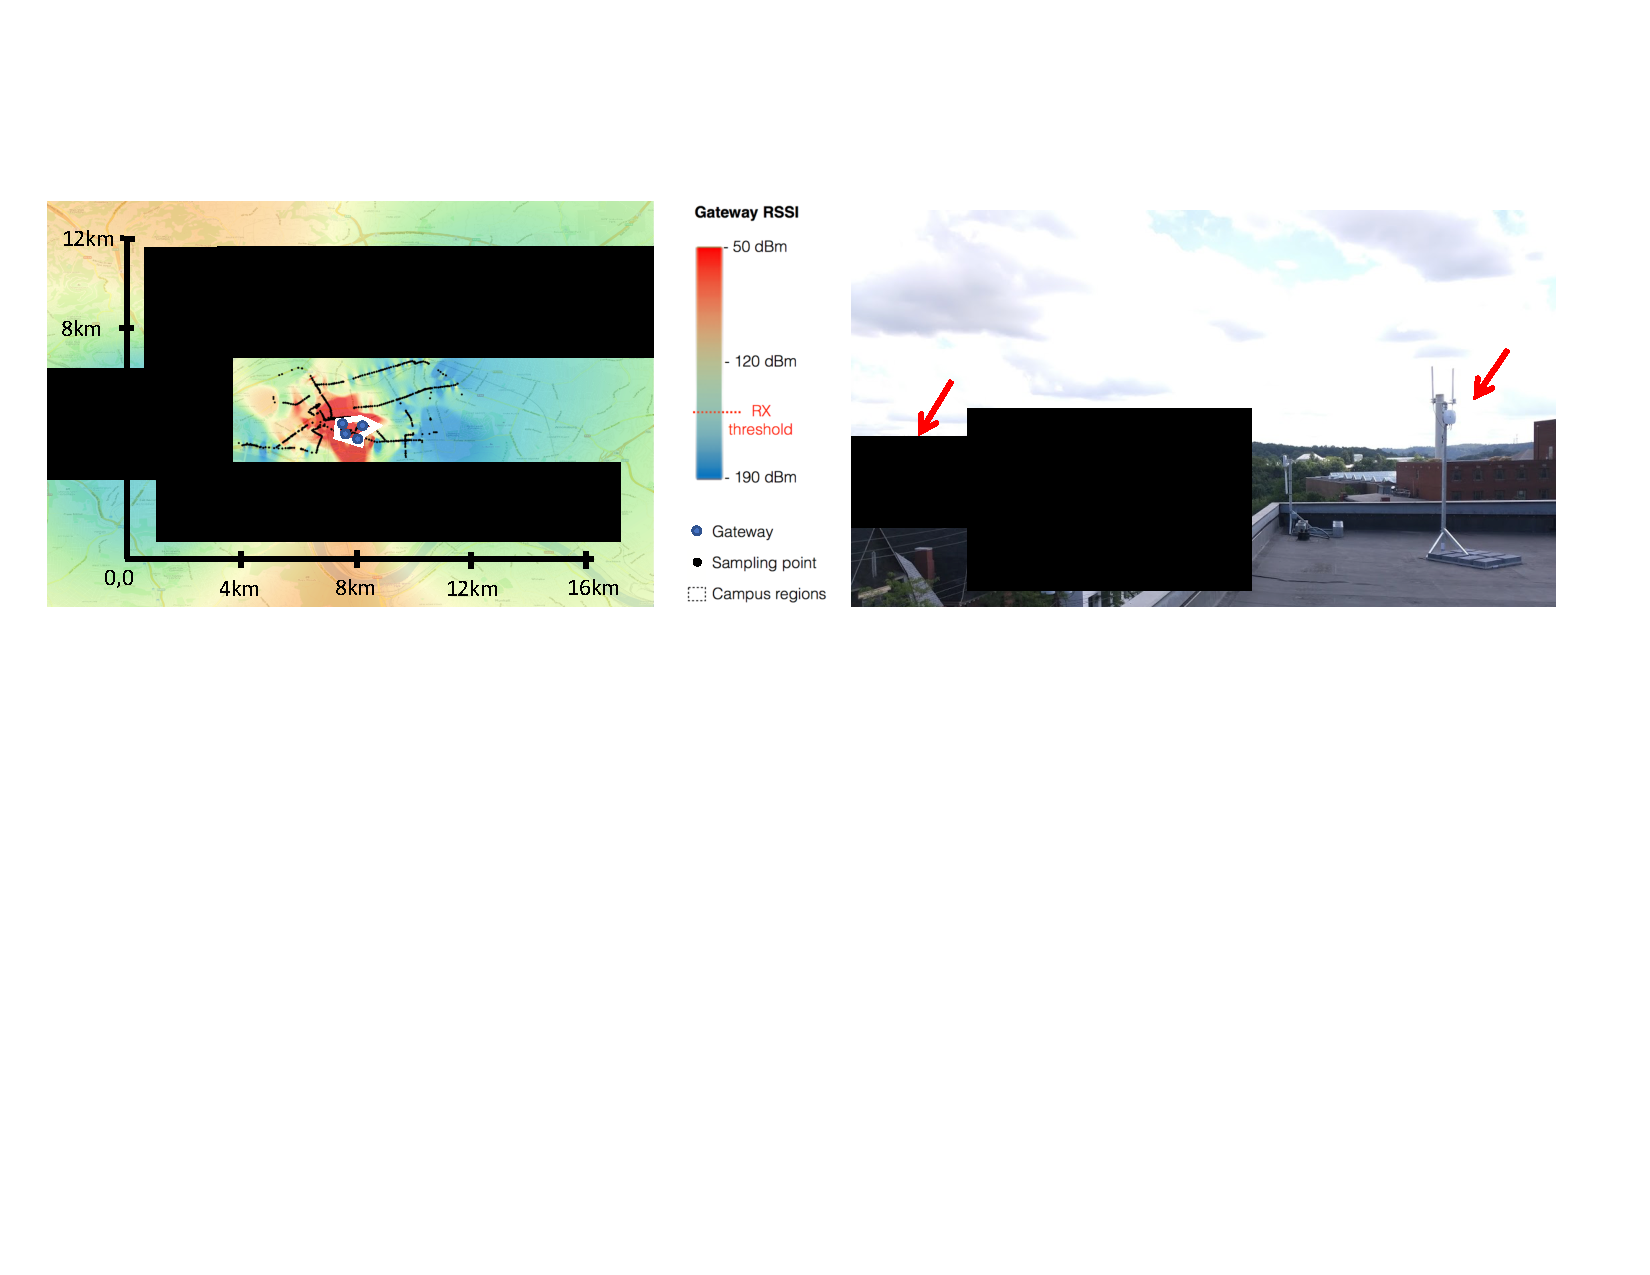
\includegraphics[width=0.9\textwidth]{figures/deployment.pdf}
    \caption{Deployment photos and coverage heat maps}
    \label{fig:deployment}
\end{figure*}

Charm is implemented as a service running on a campus-wide LoRaWAN network installed at anonymous University.  We currently have four gateways mounted on rooftops providing wide area coverage and numerous auxiliary indoor gateways extending coverage into remote parts of campus.  The LoRaWAN network is powered by the open-source Anonymous framework that allows students and faculty to login with their campus accounts and create device endpoints for capturing and sharing data.  Anonymous provides services that can be attached to data streams that can perform operations ranging from basic data storage to binary-to-json packing and unpack. A RESTful interface is used to configure meta-information about devices and set access control privileges that define how other users can interact with data streams.  The only modifications required to make a gateway Charm enabled is the additional hardware platform for receiving raw I/Q streams and a modified LoRaWAN packet forwarder that runs the packet reception event detector, maintains a circular buffer of I/Q streams and brokers interactions with the Charm cloud.  Communication between gateways and the cloud is managed using the Anonymous's MQTT publish subscriber messaging layer.

\figref{deployment}  shows examples of our gateway hardware deployed in the field along with the coverage in and around campus.  The network is currently supporting a wide-range of applications from student projects, study-space monitoring, and building occupancy sensing all the way to mechanical room environmental sensing and utility sub-metering for the campus facilities maintenance team.  The figure also shows an example coverage heat map generated by nodes deployed throughout campus and the neighboring area.  We see that the network with just four outdoor gateways is able to cover almost 10$km^2$ of urban space.

